\documentclass[10pt]{beamer}

\usepackage[utf8]{inputenc}
\usepackage[T1]{fontenc}
\usepackage{tikz}
\usepackage{hyperref}
\usepackage{array}
\usepackage{tabularx}
\usepackage{natbib}
\usetikzlibrary{calc}
\usetheme{default}



\usepackage[french]{babel}
\usepackage{amsmath,amssymb}
\usepackage{graphicx}
\usepackage{subcaption}
\usepackage{ragged2e}
\usepackage{hyperref}
\usepackage{geometry}
\usepackage{amsfonts}
\usepackage[justification=centering]{caption}
\usepackage{xcolor}
\DeclareCaptionFormat{sanslabel}{#3}
\usepackage{appendix}
\usepackage[T1]{fontenc}
\usepackage{listings}
\usepackage{picture}


\setbeamersize{
  text margin left = 1 cm, % normalement c'est 1 cm
  text margin right = 1 cm % normalement c'est 1 cm
}


\setbeamertemplate{bibliography entry article}{}
\setbeamertemplate{bibliography entry title}{}
\setbeamertemplate{bibliography entry location}{}
\setbeamertemplate{bibliography entry note}{}
\setbeamertemplate{bibliography item}[text]


\definecolor{bleu_saphir}{RGB}{31,56,85} %RAL 5003 Bleu saphir

\setbeamerfont{footline}{size=\Large}
\setbeamertemplate{footline}[frame number]
\setbeamertemplate{navigation symbols}{}
\setbeamertemplate{blocks}[rounded]
\setbeamercolor{block title}{bg=bleu_saphir!50,fg=bleu_saphir}
\setbeamercolor{block body}{bg=bleu_saphir!30,fg=bleu_saphir}
\setbeamercolor{frametitle}{fg=bleu_saphir}
\usecolortheme[named=bleu_saphir]{structure}





\addto\captionsfrench{%
  \renewcommand{\figurename}[1]
        {{\textit{#1}}}}
\addto\captionsfrench{%
  \renewcommand{\subfigurename}[1]
        {{\textit{#1}}}}
\newcommand{\saut}{\vspace{10pt}}
\definecolor{pbblue}{rgb}{100,100,100}% color for the progress bar and the circle

\makeatletter
\def\progressbar@progressbar{} % the progress bar
\newcount\progressbar@tmpcounta% auxiliary counter
\newcount\progressbar@tmpcountb% auxiliary counter
\newdimen\progressbar@pbht %progressbar height
\newdimen\progressbar@pbwd %progressbar width
\newdimen\progressbar@rcircle % radius for the circle
\newdimen\progressbar@tmpdim % auxiliary dimension

\progressbar@pbwd=300pt
\progressbar@pbht=1pt
\progressbar@rcircle=2.5pt

% the progress bar
\def\progressbar@progressbar{%
\hspace{-200pt}
    \progressbar@tmpcounta=\insertframenumber
    \progressbar@tmpcountb=\inserttotalframenumber
    \progressbar@tmpdim=\progressbar@pbwd
    \multiply\progressbar@tmpdim by \progressbar@tmpcounta
    \divide\progressbar@tmpdim by \progressbar@tmpcountb

  \begin{tikzpicture}[remember picture,overlay]
    \draw[pbblue!100,line width=\progressbar@pbht]
      (-150pt, 6pt) -- ++ (\progressbar@pbwd,0pt);

    \filldraw[pbblue!100] %
      (\the\dimexpr\progressbar@tmpdim-\progressbar@rcircle\relax-150pt,6pt) circle (\progressbar@rcircle);
  \end{tikzpicture}%
}

\addtobeamertemplate{footline}{}
{%
  \begin{beamercolorbox}[wd=\paperwidth,ht=4ex,center,dp=1ex]{white}%
    \progressbar@progressbar%
  \end{beamercolorbox}%
}
\makeatother

\usepackage{listings}
\usepackage{xcolor}
\usepackage{amsmath}
 
\definecolor{codegreen}{RGB}{161,194,128}
\definecolor{codegray}{RGB}{128,128,128}
\definecolor{codepurple}{RGB}{186,125,214}
\definecolor{backcolour}{RGB}{41,43,51}
\definecolor{codenumber}{RGB}{199,156,110}
\definecolor{codeblue}{RGB}{115,173,232}
\definecolor{codeblue2}{RGB}{86,182,194}
 
\lstdefinestyle{styleC}{
    language=C,
    backgroundcolor=\color{backcolour},
    commentstyle=\color{codegray},
    keywordstyle=\color{codepurple},
    keywordstyle=[2]\color{codenumber},
    keywordstyle=[3]\color{codeblue},
    numberstyle=\tiny\color{codegray},
    stringstyle=\color{codegreen},
    basicstyle=\ttfamily\footnotesize\color{white},
    breakatwhitespace=false,
    breaklines=true,
    captionpos=b,
    keepspaces=true,
    numbers=left,
    numbersep=5pt,
    showspaces=false,
    showstringspaces=false,
    showtabs=false,
    tabsize=4,
    otherkeywords={0,1,2,3,4,5,6,7,8,9,main,printf,*,gradient,descente,malloc,objectif,free,integrale},
    morekeywords=[2]{0,1,2,3,4,5,6,7,8,9},
    morekeywords=[3]{main,printf,gradient,descente,malloc,objectif,free,integrale}
}

\lstdefinestyle{stylePython}{
    language=Python,
    backgroundcolor=\color{backcolour},
    commentstyle=\color{codegray},
    keywordstyle=\color{codepurple},
    keywordstyle=[2]\color{codenumber},
    numberstyle=\tiny\color{codegray},
    stringstyle=\color{codegreen},
    basicstyle=\ttfamily\footnotesize\color{white},
    breakatwhitespace=false,
    breaklines=true,
    captionpos=b,
    keepspaces=true,
    numbers=left,
    numbersep=5pt,
    showspaces=false,
    showstringspaces=false,
    showtabs=false,
    tabsize=4,
    otherkeywords={0,1,2,3,4,5,6,7,8,9,range,len},
    morekeywords=[2]{0,1,2,3,4,5,6,7,8,9},
}


\usebackgroundtemplate{
\includegraphics[width=\paperwidth,height=\paperheight]{template_lmps_titre_43.png}}

\title{\textcolor{bleu_saphir}{\textbf{Aménagement d'infrastructures pour la livraison à domicile}}}
\author{\textcolor{bleu_saphir}{\textbf{BIOULAC Jules}}}

\date{\textcolor{bleu_saphir}{13335}}


\begin{document}


\begin{frame}[noframenumbering]

    \vspace{100pt}
    \maketitle
    \setbeamertemplate{footline}{}

\end{frame}


\usebackgroundtemplate{
\includegraphics[width=\paperwidth,height=\paperheight]{template_lmps_43.png}}

\begin{frame}{\textbf{Mise en situation}}

    \begin{itemize}
        \item Les \textbf{transports} sont la plus grosse source d'émissions de \textbf{GES} en France
        \item La livraison à domicile est un processus qui coûte \textbf{de plus en plus cher} à mesure qu'on se rappoche de la fin
    \end{itemize}

\end{frame}


\begin{frame}{\textbf{Mise en situation}}
    
    \begin{itemize}
        \item \textbf{Livraison à domicile} : Le client \underline{reçoit} son colis à son \textit{domicile}
        \begin{itemize}
            \item \textit{Simplicité} : le client n'a pas à se déplacer pour récupérer son colis
        \end{itemize}
    \end{itemize}
    \vspace{15pt}
    \begin{itemize}
        \item \textbf{Livraison en point relais} : Le client va \underline{chercher} son colis dans un \textit{point relais}
        \begin{itemize}
            \item \textit{Coût} : le coût de la livraison est plus faible
            \item \textit{Flexibilité} : le client peut choisir quand aller récupérer son colis
        \end{itemize}
    \end{itemize}

\end{frame}


\begin{frame}{\textbf{Problématique}}

    $\longrightarrow$ \textbf{Comment répartir les points de retrait de colis au sein d'une ville ?}

\end{frame}


\begin{frame}{\textbf{Sommaire}}

    %\tableofcontents
    \tableofcontents[hideothersubsections]

\end{frame}


\section{Formalisation du problème}
\begin{frame}{\textbf{Formalisation du problème}}

    \begin{itemize}
        \item On se place dans le carré \textbf{[0,1]x[0,1]}
        \item Chaque \textbf{point} du carré représente un potentiel \textbf{client}
        \item Il s'agit de placer les \textbf{points de retrait} pour minimiser :
        \begin{itemize}
            \item Distance moyenne à un point
            \item Nombre de points de retrait
        \end{itemize}
    \end{itemize}

\end{frame}


\begin{frame}{\textbf{Formalisation du problème}}

    \begin{itemize}
        \item La \textbf{distance} d'un client aux points de retrait est celle au point de retrait le plus proche
    \end{itemize}
    $$dist(x_0, y_0, points) := \underset{(x, y)\in{}points}{min} \sqrt{(x_0-x)^2 + (y_0-y)^2}$$
    \newline
    \begin{itemize}
        \item La \textbf{distance moyenne} est alors la fonction \textit{objectif} :
    \end{itemize}
    $$objectif(points) := \int_{0}^{1}\int_{0}^{1} dist(x, y, points) ~dx~dy$$

\end{frame}


\section{Premiers tests}
\begin{frame}{\textbf{Premiers tests}}

    \begin{itemize}
        \item Algorithme d'optimisation :
        \begin{itemize}
            \item Descente de gradient
            \item Algorithmes mimétiques
        \end{itemize}
    \end{itemize}

\end{frame}


\begin{frame}{\textbf{Premiers tests}}

    \begin{center}
        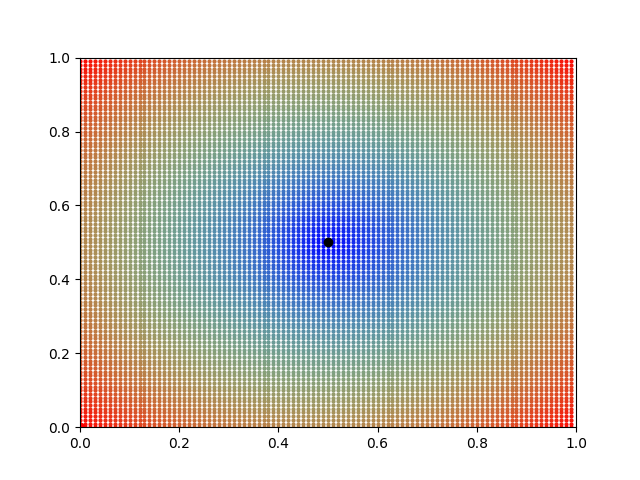
\includegraphics[height=5cm, width=5cm]{../../Figure_1pt_0att.png}
        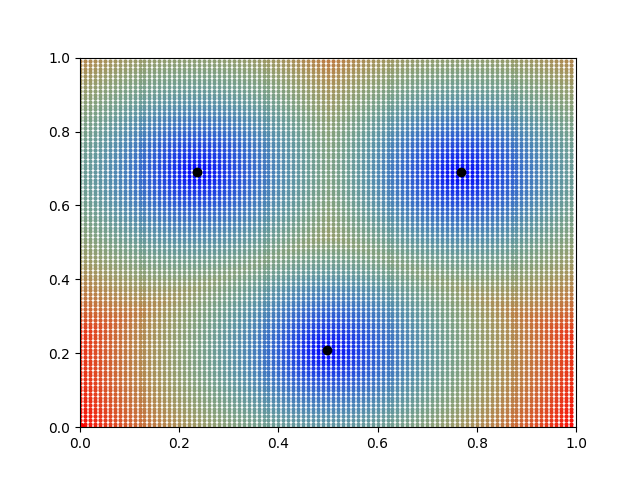
\includegraphics[height=5cm, width=5cm]{../../Figure_3pt_0att.png}
    \end{center}

\end{frame}


\section{Que sont les attracteurs ?}
\begin{frame}{\textbf{Que sont les attracteurs ?}}

    \begin{itemize}
        \item Représentent les différents besoins
        \item Choix : Revenu moyen
        \begin{itemize}
            \item \textbf{INSEE} : Corrélation
        \end{itemize}
        \item On choisit alors les attracteurs :
        \begin{itemize}
            \item 1 attracteur = 1 arrondissement de Paris
            \item Coefficient $\propto$ revenu moyen
        \end{itemize}
    \end{itemize}

\end{frame}


\section{Ajout des attracteurs}
\begin{frame}{\textbf{Ajout des attracteurs}}

    Objectif des attracteurs :
    \begin{itemize}
        \item Représenter les différents besoins
    \end{itemize}
    
    \lstset{style=styleC}
    \lstinputlisting[firstline=10, lastline=15]{../../Projet/attracteur.c}

\end{frame}


\begin{frame}{\textbf{Ajout des attracteurs}}

    \begin{itemize}
        \item Il faut alors les prendre en compte dans le \textbf{calcul de la distance}
        \item On va alors \textbf{multiplier} chaque distance par un \textbf{coefficient} prédéfini qui dépend des coefficients des attracteurs
        \item Pour un point $(x_0, y_0)$, on note $coeff(x_0, y_0, attracteurs)$ le coefficient associé
    \end{itemize}

\end{frame}


\begin{frame}{\textbf{Ajout des attracteurs}}

    \begin{itemize}
        \item La distance devient alors
    \end{itemize}
    $$dist(x_0, y_0, points, attracteurs) := $$
    $$coeff(x_0, y_0, attracteurs)\times\underset{(x, y)\in{}points}{min} \sqrt{(x_0-x)^2 + (y_0-y)^2}$$
    $$$$

    \begin{itemize}
        \item La distance moyenne change également
    \end{itemize}
    $$objectif(points, attracteurs) := $$
    $$\int_{0}^{1}\int_{0}^{1} dist(x, y, points, attracteurs) dxdy$$

\end{frame}


\begin{frame}{\textbf{Ajout des attracteurs}}
    
    \begin{itemize}
        \item Dans notre cas, pour $(x_0, y_0)$
        \begin{itemize}
            \item Attracteur le plus proche : $(x_a, y_a, c_a)$
            \item $d := \sqrt{(x_0-x_a)^2 + (y_0-y_a)^2}$
            \item On utilise alors
        \end{itemize}
    \end{itemize}
    $$coeff(x_0, y_0, attracteurs) := c_a*e^{\frac{-1}{(\sqrt{2}-d)^5}}$$

\end{frame}


\section{Calcul des coefficients}
\begin{frame}{\textbf{Calcul des coefficients}}

    \begin{center}
        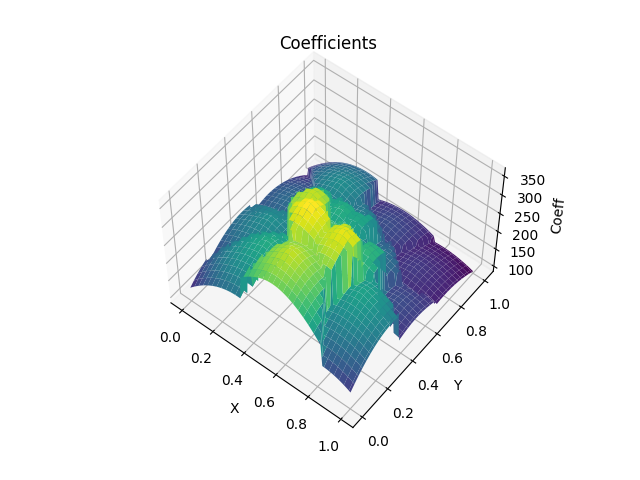
\includegraphics[height=10cm, width=10cm, keepaspectratio=true]{../../Figure_Coeff.png}
    \end{center}

\end{frame}


\section{Résultats avec les attracteurs}
\begin{frame}{\textbf{Résultats avec les attracteurs}}

    \begin{center}
        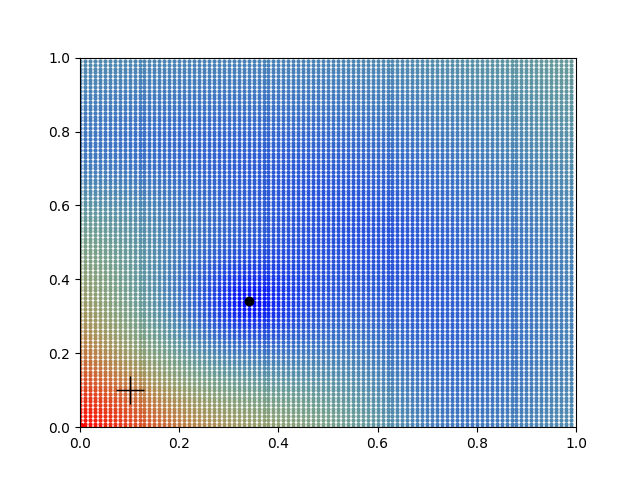
\includegraphics[height=7.5cm, width=7.5cm]{../../Figure_1pt_1att5.png}
    \end{center}

\end{frame}


\begin{frame}[noframenumbering]{\textbf{Résultats avec les attracteurs}}

    \begin{center}
        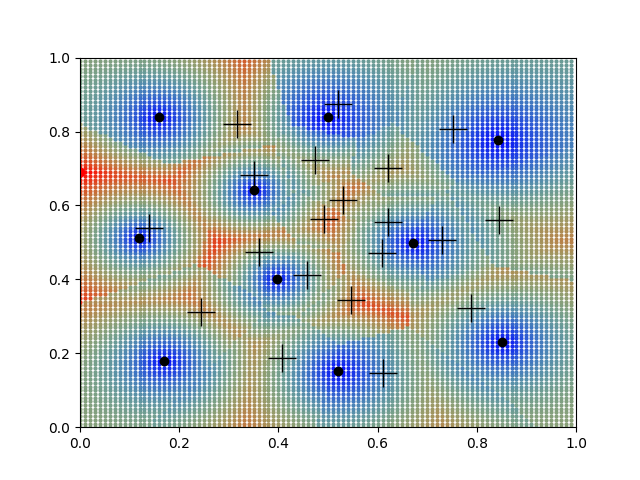
\includegraphics[height=7.5cm, width=7.5cm]{../../Figure_10pt_paris.png}
    \end{center}

\end{frame}


\section{Pistes d'amélioration}
\begin{frame}{\textbf{Pistes d'amélioration}}

    \begin{itemize}
        \item Manque de puissance de calcul
        \begin{itemize}
            \item Comparaison résultats avec réalité
        \end{itemize}
        \item Prise en compte densité de population
        \item Descente de gradient optimale ?
    \end{itemize}

\end{frame}


\end{document}